\section{Algorytm Neville'a}
\begin{frame}
{3.6 Algorytm Neville'a}

O algorytmie Neville'a: Data Analysis BriefBook5 (autor: Rudolf K. Bock,CERN)
{\it http://www.cern.ch/RD11/rkb/AN16pp/node182.html} \newline

\textcolor{blue}{Istota:} budowa tablicy wielomianów coraz wyższych stopni.
\begin{figure}[h]
			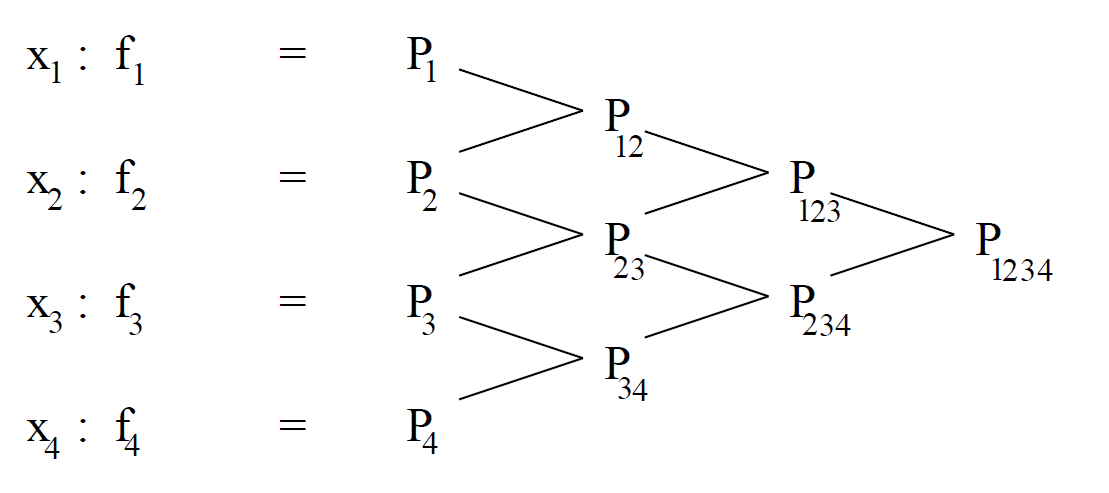
\includegraphics[scale = 0.28]{img/3/interpol_3_6}
	\end{figure}
Rysunek 3.3: Ilustracja metody Neville'a
\end{frame}

\begin{frame}
$P_{1}, P_{2}, P_{3}, P_{4}$ -- wiel. stopnia $0$, przechodzący przez $(x_{i},\ f_{i})$ ,

$P_{12}, P_{23}, P_{34}$ -- wartość w $x$ dla wielomianów stopnia 1, przechodzącego przez pary punktów, \\
\vspace{4mm}
\textbf{Rekurencyjne zapełnianie tabeli:}
\begin{gather*}
	P_{i(i+1)\ldots(i+m)}=\\
	=\displaystyle \frac{(x-x_{i+m})P_{i(i+1)\ldots(i+m-1)}+(x_{i}-x)P_{(i+1)(i+2)\ldots(i+m)}}{x_{i}-x_{i+m}}
\end{gather*}

\begin{itemize}
\item Otrzymamy wielomian stopnia $N-1$

\item Zgodny z $f(x)$ w węzłach, np.:
$$
P_{12}=\frac{(x-x_{2})P_{1}-(x-x_{1})P_{2}}{x_{1}-x_{2}}\ ;\ P_{12}(x_{1})=P_{1};P_{12}(x_{2})=P_{2}
$$

\end{itemize}

\end{frame}

\begin{frame}


Wygodniej-- różnice między pokoleniami:
$$
C_{m,i}=P_{i\cdots(i+m)}-P_{i\cdots(i+m-1)}\ ;\ D_{m,i}=P_{i\cdots(i+m)}-P_{i\cdots(i+m)}
$$
$$
D_{m+1,i}\ =\ \frac{x_{i+m+1}-x}{x_{i}-x_{i+m+1}}(C_{m,i+1}-D_{m,i})
$$
$$
C_{m+1,i}\ =\ \frac{x_{i}-x}{x_{i}-x_{i+m+1}}(C_{m,i+1}-D_{m,i})
$$
\vspace{3mm}

Końcowy wynik -- suma różnic wzdłuż wybranej ścieżki. \\
Dodatkowo otrzymujemy oszacowanie błędu. \\
\vspace{3mm}
\textbf{Zadanie}: sprawdzić poprawność, napisać algorytm, \\
oszacować błąd.
\end{frame}
